\documentclass[11pt]{article}
\usepackage{latexsym}
\usepackage{graphicx}
\usepackage{amsmath,amssymb,amsthm,calc}
\usepackage{euscript}
\usepackage{mathpazo}
\usepackage{mathtools}
\usepackage{tabularx}
\usepackage{bm}
\usepackage{makecell}

\usepackage[linesnumbered,lined,boxed,commentsnumbered]{algorithm2e}

\usepackage[top=1.25in,bottom=1.25in,left=2in,right=2in]{geometry}
\usepackage{enumitem}
\newlist{steps}{enumerate}{1}
\setlist[steps, 1]{leftmargin=3\parindent, label = Step \arabic*:}


\usepackage{subfig}
\usepackage{microtype}
\usepackage{fullpage}
\usepackage{xspace}
\usepackage{tikz,color}  % Used for the extended footnotes if needed
\definecolor{newblue}{rgb}{0.2,0.2,0.6}
\usepackage[colorlinks,allcolors=newblue]{hyperref}
\newcommand*{\vertbar}{\rule[-1ex]{0.5pt}{2.5ex}}
\newcommand*{\horzbar}{\rule[.5ex]{2.5ex}{0.5pt}}
\DeclareMathOperator{\E}{\mathbb{E}}

\newcommand{\handout}[5]{
   \renewcommand{\thepage}{#1-\arabic{page}}
   \noindent
   \begin{center}
   \framebox{
      \vbox{
    \hbox to 5.78in { {\bf MATH 690: Topics in Probablity Theory} \hfill #2 }
       \vspace{4mm}
       \hbox to 5.78in { {\Large \hfill #5  \hfill} }
       \vspace{2mm}
       \hbox to 5.78in { {\it #3 \hfill #4} }
      }
   }
   \end{center}
   \vspace*{4mm}
}

\renewcommand{\paragraph}[1]{\medskip \noindent {\bf #1.}}

\newcommand{\lecture}[4]{\handout{#1}{#2}{Lecturer: #3}{Scribe: #4}{#1}}
\DeclarePairedDelimiter\floor{\lfloor}{\rfloor}
\newcommand{\norm}[1]{\left\lVert#1\right\rVert}
\theoremstyle{definition}
\newtheorem{definition}{Definition}
\newtheorem{remark}{Remark}
\newtheorem{theorem}{Theorem}
\newtheorem{lemma}[theorem]{Lemma}
\newtheorem{corollary}{Corollary}
\newtheorem{fact}[theorem]{Fact}
\newtheorem{observation}[theorem]{Observation}
\newtheorem{excercise}{Excercise}
\newtheorem{Example}{Example}

\newcommand{\example}[1]{\paragraph{Example #1}}

\begin{document}
\lecture{Dimension Reduction}{September 14, 19, 2017}{Xiuyuan Cheng}{Fred Zhang}
\section{Introduction}
In this lecture, we continue to discuss covariance estimation. We observe the Stein's phenomenon when MLE is suboptimal and develop the methods of \textit{spectral shrinkage} and covariance thresholding. We then turn to dimension reduction and consider the \textit{Multidimensional Scaling} (MDS) problem, which is equivalent of PCA.

\section{Stein's Phenomenon}
Let us wrap up our previous discussion on the Stein's phenomenon.  Suppose we a one dimensional random variable $y\sim \mathcal{N}(\mu,1)$; that is $p=1$, $n=1$. Given only one observation, we want to estimate the mean $\mu$. It is easy to see that the Maximum Likelihood Estimator is 
\[
    \widehat{\mu}^{MLE} (y) = y.
\]
Can we construct better ones, and how do we evaluate an estimator? For that purpose we consider the \textit{Mean Squared Error} (MSE) of an estimator, defined as
\[
    \E\left(\widehat{\mu} - \mu\right)^2 = \underbrace{\E\left(\widehat{\mu} -\mu\right)^2}_{\text{variance}} + \underbrace{\left(\E \widehat{\mu} - \mu\right)^2}_{\text{bias}^2}.
\]
Notice that the first term  is the variance and the second is the bias squared (of the estimator). Now based on this definition, we see that the MSE of the MLE is
\[
    \E \left(\widehat{\mu}^{MLE}-\mu\right)^2 = 1+ 0 =1.
\]
Can we have another estimator that has less MSE\@? Let us consider $\widehat{\mu}(u) = \rho \cdot y$ for some $\rho$ to be determined. Then its MSE is
\[
    \E \left(\widehat{\mu} -\mu\right)^2 = \rho^2 + (\rho-1)^2 \mu^2.
\]
Here, we calculate that the minimizer of the RHS, a quadratic polynomial in $\rho$, is
\[
\rho^* = \frac{\mu^2}{1+\mu^2}.
\]
Hence, MLE is suboptimal in terms of the MSE\@. To construct a better estimator, we should, in this case, {\it shrink}\ it by some factor $\rho$, although its optimal choice can be unknown to us. The question is how we should do this in general setting.

\subsection{Spectral Shrinkage}
In covariance estimation of high dimensions, what we shall consider is the {\it spectral shrinkage}\ on the eigenvectors. Last time we saw the BBP phase transition of the spiked model in rank-$1$ case, where if $R$ is the signal-noise ratio, then the largest eigenvalue converges  to $1+R$. The transition threshold occurs at $\sqrt{\gamma}$, where $\gamma = p/n$.
\begin{figure}[htbp]
    \centering
    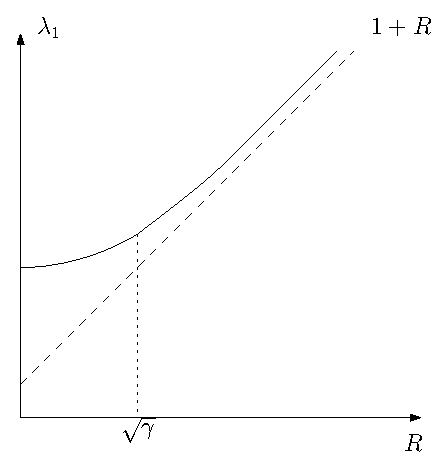
\includegraphics[scale=.85]{./fig/bbp.eps}
    \caption{The largest eigenvalue starts to approach to $1+R$ at $R= \sqrt{\gamma}$.}
\end{figure}

In general, eigenvectors corresponding to eigenvalues below certain threshold come from noise. Now consider the eigendecomposition of the covariance matrix $\mathbf{S_y} = \mathbf{V}\bm{\Lambda} \mathbf{V}^T$. We intend to estimate the population covariance matrix by  applying a {\it shrinkage function} $f$:
\[
    \bm{ \widehat{\Sigma} }= \mathbf{V}f(\bm{\Lambda})\mathbf{V}^T = \sum_{i=1}^p f(\bm{\Lambda_i})\mathbf{v_i} \mathbf{v_i}^T.
\]
Here, we would choose some thresholding function $f$ that filters out small eigenvalues; \textit{e.g.},
\begin{figure}[htbp]
    \centering
    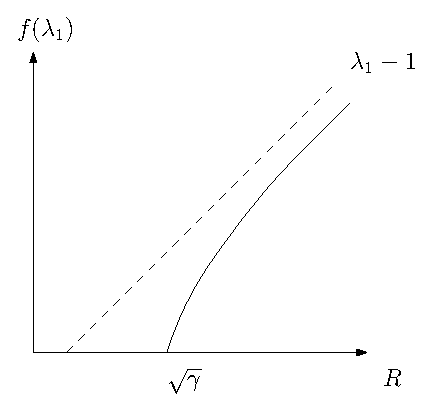
\includegraphics[scale=.90]{./fig/shrink.eps}
    \caption{Shrinkage function.}
\end{figure}

\subsection{Thresholding Sample Covariance}
Now we introduce another method for denoising the sample covariance and estimate the population covariance. Let $\mathbf{S}= \frac{1}{n}\sum_{i}\mathbf{y_i}\mathbf{y_i}^T$ be the sample covariance. Then simply apply a thresholding function: $$\widehat{\Sigma}_{ij} = Tr(S_{ij}).$$ Here, the function $Tr(\cdot)$ is 
\begin{figure}[htbp]
    \centering
    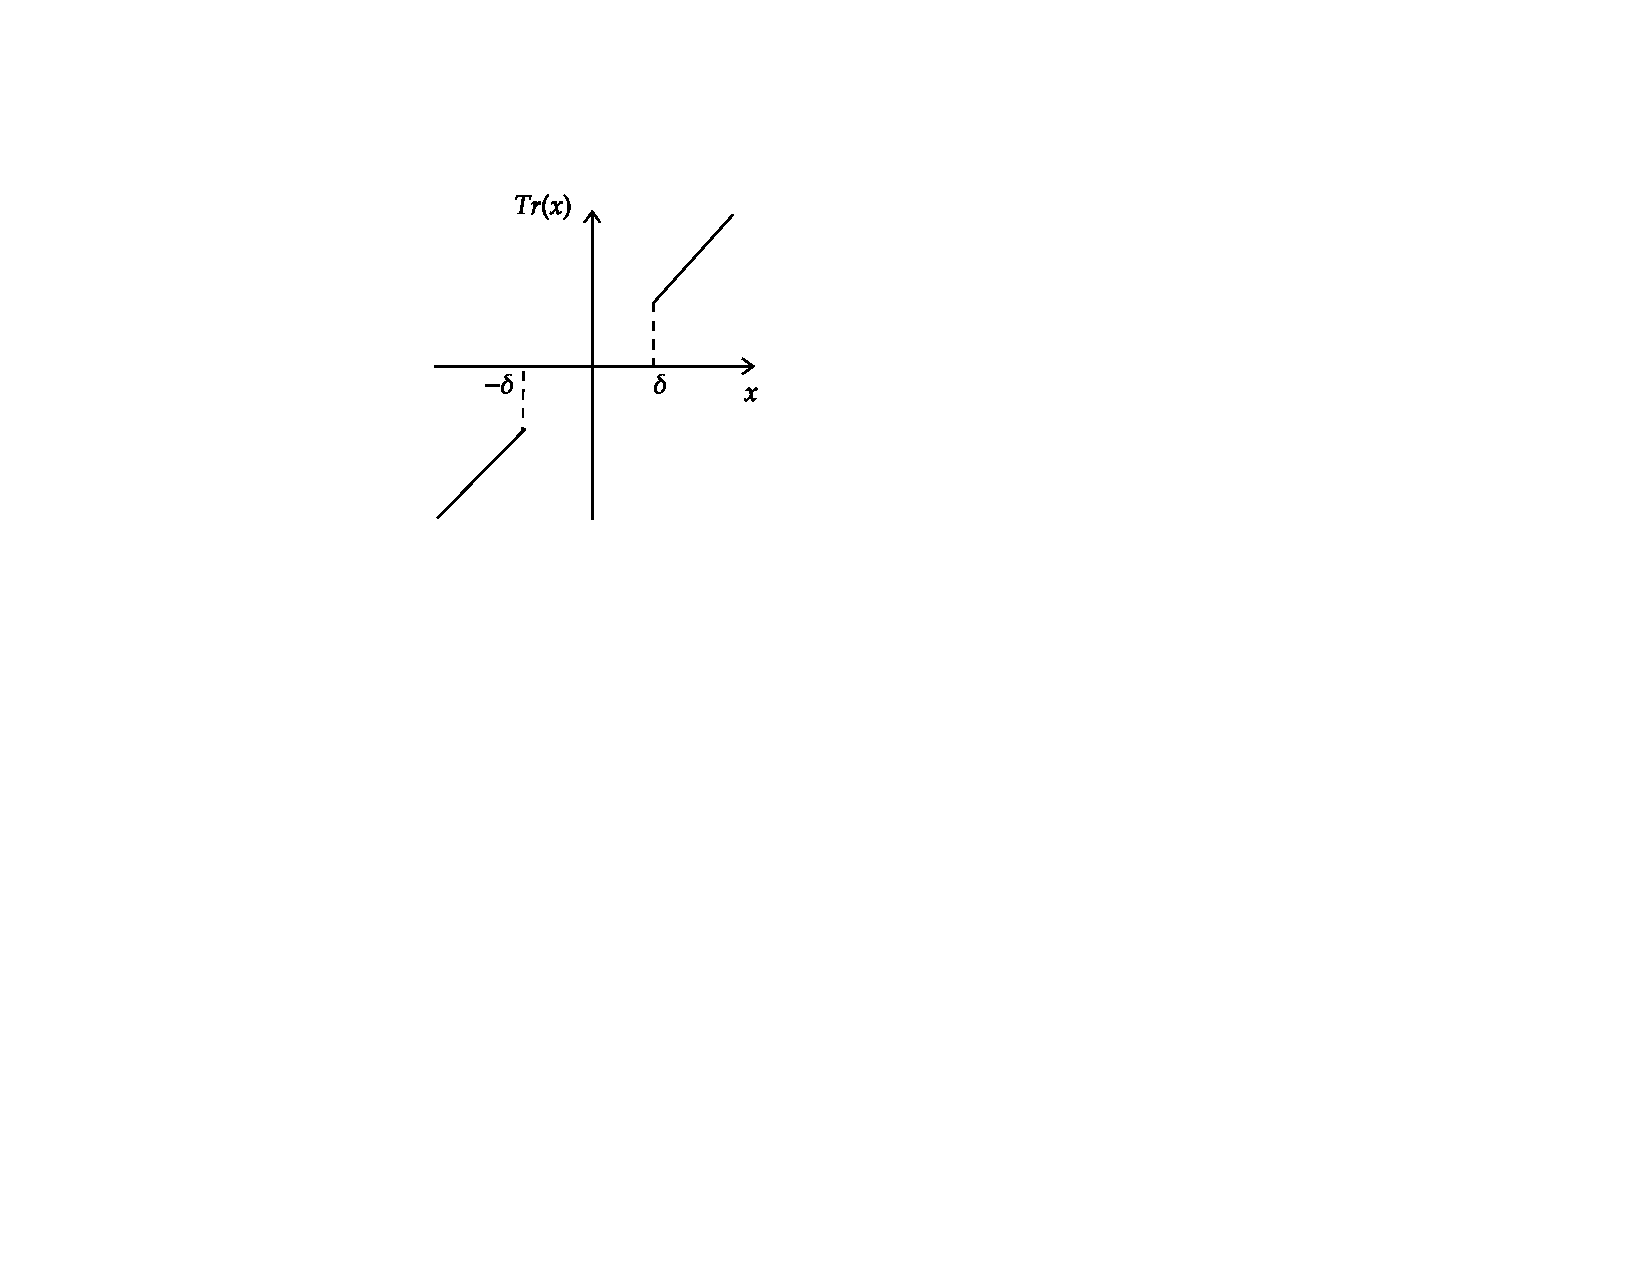
\includegraphics[scale=.85]{./fig/tr.pdf}
    \caption{Thresholding function $Tr(x)$.}
\end{figure}

That is, we filter out entries of small absolute values.
\begin{excercise}
    Let $y_i\sim \mathcal{N}(0,1)$ be i.i.d.\ Gaussian samples. After applying the thresholding function with $\delta = \frac{2\log n}{\sqrt{n}}$ on the sample covariance,  non-diagonal entries converge to $\mathcal{N}(0,c/n)$ as $n\rightarrow \infty$, for some constant $c$. Roughly speaking, only diagonal entries remain.
\end{excercise}

For more on the thresholding method and its theoretical justification, see~\cite{bickel2008covariance}. This is also related to the whole area of Sparse PCA; see~\cite{johnstone2009consistency}.

\section{Introduction to Dimension Reduction}
Given $\left\{\mathbf{x_i} \in \mathbb{R}^D\right\}_{i=1}^n$. For the purpose of faster algorithms, visualization, \textit{etc.}, we  would like to  to have another set of points  $\left\{\mathbf{y_i}\in\mathbb{R}^d\right\}_{i=1}^n $ with $d\ll D$. We want that the ``geometry'' of $\{\mathbf{x_i}\}$ are as much preserved as possible in $\{\mathbf{y_i}\}$. Can we do it in general, say, to preserve distances between $\{\mathbf{x_i}\}$?
\begin{Example}
    Suppose $D=3$, $d=2$ and $n=3$. Take the hyperplane the three points lie on. It is easy to see that we can embed them in $\mathbb{R}^2$ without distorting pairwise distances.
\end{Example}
\begin{Example}
    Suppose $D=3$, $d=2$ and $n=4$. If the four points do not lie on the same hyperplane, then it is not possible to preserve the pairwise distances in $\mathbb{R}^2$.
\end{Example}
Hence, it not possible to always preserve metrics in reducing dimensions. However, we also observed that if the data lie on a subspace, then finding the subspace can give us a low dimension embedding. Next, we will discuss how to do this under Euclidean distances.

\section{Multidimensional Scaling (MDS)}
Given $\mathbf{X} = [\mathbf{x_1},\ldots,\mathbf{x_n}]_{D\times n}$, we would like to find $\mathbf{Y}= [\mathbf{y_1},\ldots, \mathbf{y_n}]_{d\times n}$ that minimize the discrepancies $L(Y)$
\begin{equation}\label{eqn:otp}
    \min L(\mathbf{Y}) = \sum_{i,j} \left(\norm{\mathbf{y_i}-\mathbf{y_j}}^2-\underbrace{\norm{\mathbf{x_i}-\mathbf{x_j}}^2}_{D_{ij}}\right)^2.
\end{equation}
Without loss of generality, assume that input data are centered at origin (\textit{i.e.}, $\sum \mathbf{x_i} = \mathbf{0}$ and $\mathbf{X}\cdot \mathbf{1} = \mathbf{0}$).  Let $$D_{ij} = \norm{\mathbf{x_i}-\mathbf{x_j}}^2 = \norm{\mathbf{x_i}}^2 + \norm{\mathbf{x}}_j^2 - 2\mathbf{x_i}^T\mathbf{x_j}.$$ Then it can be expressed as
\[
    \mathbf{D} = \bm{\xi}\mathbf{1}^T +  \mathbf{1}\bm{\xi}^T - 2\bm{G}, 
\]
where $\mathbf{G} = \mathbf{X}^T\mathbf{X}$ is the Gramian and $\bm{\xi} = \left[\norm{\mathbf{x_i}}^2 , \ldots, \norm{\mathbf{x_n}}^2\right]^T$. In general, the input is not necessarily $\mathbf{X}$ but only the distance matrix $\mathbf{D}$. This problem is in fact equivalent of PCA\@. However, one can still compute the Gramian without not knowing the data coordinates $\mathbf{X}$ by \textit{double centering}.

Let $\bm{H} = \bm{I} - \frac{1}{n}\bm{1}\bm{1}^T$. We notice that since $\bm{H \cdot 1} =\bm{0}$, $\bm{HGH} = \mathbf{H}(\bm{X}^T\bm{X})\bm{H} = G$. Then
\[
    - \frac{1}{2}\bm{HDH} = \bm{G}.
\]
We obtain $\bm{Y}$, we compute $\mathbf{\widetilde{G}}$ by applying PCA on $\bm{G}$ using the top $k$ eigenvectors. It turns out that setting $\bm{Y} = \bm{S}_{1:d,1:d} \bm{V}_{:,1:d}$ minimizes the objective~(\ref{eqn:otp}).

\section{Isomap}
Given $\mathbf{X} = [\mathbf{x_i}]_{D\times n}$, we want to embed them in lower dimension by finding $\mathbf{Y}= [\mathbf{y_i}]_{d\times n}$.
\begin{steps}
\item Graph construction. Construct a $k$-NN graph such that $A_{ij}=1 $ if $i\in N(j)$ and (or) $j\in N(i)$ and $A_{ij} =0$ otherwise. Here, $N(i)$ is a list of $k$ nearest neighbors in Euclidean distance. As an alternative, one constructs $\epsilon$-graph where $A_{ij}=1$  iff $\norm{\bm{x_i}-\bm{x_j}} < \epsilon$. 
    \item  Compute graph distance. Compute shortest-path distance $d_{ij}$ for all pairs $i,j$ in the graph 
    \item Classical MDS\@. Compute $D_{ij} =d^2_{ij}$, the Gramian $\bm{G}=-\frac{1}{2}\bm{HDH}$, then compute the top $d$ eigenvectors of $G$.
\end{steps}
\begin{remark}
    If the data sit on some low-dimensional manifold, under certain assumptions ({\it e.g.}, on sampling of the points), the shortest path distance we compute approximates the geodesic distance on the manifold.
\end{remark}
\begin{remark}
The decay of the eigenvalues of $G$ can indicate the intrinsic dimension of the data.
\end{remark}

\section{Locally Linear Embedding (LLE)} 
\begin{steps}
    \item Construct the $N(i)$ list of $k$-NN for all points.
    \item Solve least-square optimization problem
        \[
            \min _{d_j^{(i)}} \norm{x_i- \sum_{j\in N(i)} d_j^{(i)} x_j}^2
        \]
        such that $\sum_{j\in N(i)} d_j^{(i)} =1$.
    \item Compute 
        \[
            W_{ij} = \begin{cases}
                d_j^{(i)} & j\in N(i)\\
                0 & \text{otherwise}
            \end{cases}
        \]
        and 
    \[
        \min _{\bm{Y}} \sum_{i} \norm{y_i -\sum_j W_{ij}y_j}^2
    \]
    such that $\bm{Y}\bm{1}=\bm{0}$ and $\bm{Y}^T\bm{T}=\bm{I}_d$. This turns out to be an eigvenvalue problem on $\bm{M}=(\bm{I}-\bm{W})^T(\bm{I}-\bm{W})$.
\end{steps}
\begin{remark}
    The matrix $\bm{M}$ approximates the graph Laplacian $\bm{L}$ of the $k$-NN graph.
\end{remark}

\section{Laplacian Eigenmap}
\begin{steps}
\item Construct the affinity matrix $\bm{W}$ where 
    \[ 
    W_{ij} = e^{\frac{-\norm{x_i-x_j}^2}{\epsilon}}.
    \]
    As a simpler alternative, let $W$ be the adjacency matrix by the $k$-NN graph or $\epsilon$-graph
\item Compute the graph Laplacian $\bm{L} = \mathbf{D} - \bm{W}$.
\item Compute the eigendecomposition of $\bm{L_{rw}} = \bm{D}^{-1}\bm{L}$:
    \[
        \bm{L\Phi} =\bm{\lambda D \Phi}
    \]
    Then $\mathbf{Y} = [\Phi_2, \ldots, \Phi_{d+1}]$, eigvenvectors corresponding to the $2$nd and $(d+1)$st smallest eigvenvalue.
    \end{steps}
Note 
    \[
        \mathbf{L_{rw} = \bm{D}^{-1} (\bm{D}-\bm{W})} = \bm{I} - \underbrace{\bm{D}^{-1}\bm{W}}_{\bm{P}}.
    \]
    Here $P_{ij}= W_{ij} / d_i$.  We notice that $\mathbf{P}$ is a probablisitic matrix, and this defines a random walk on the graph. The eigenvalues of $\bm{P}$ are in $[-1,1]$. The largest eigenvalue is $\lambda_1 =1$ is of multiplicity $1$ if the graph is connected and $-1$ is not an eigenvalue if the random walk has not cylces.
\begin{excercise}
    What is the stationary distribution of $\bm{P}$?
\end{excercise}

\bibliographystyle{alpha}
\bibliography{bib}

\end{document}
